% TODO: make virtual box names color coded
% Insert images
\documentclass[a4paper,11pt]{article}
\usepackage{hyperref}
\usepackage{graphicx} 
\usepackage{caption}
% define the title
\author{
	Animesh Pramanik \\
	\and
	Henna Arora\\
	\and
	Sourav Goswami}
\title{ROHC Writeup}
\begin{document}
% generates the title
\maketitle
\pagebreak
% insert the table of contents
\tableofcontents
\pagebreak

\section{The ROHC framework}
About the framework and library itself, the link.
\pagebreak

\section{Deploying the library}
The types of deployment options we have.
\subsection{Using the library}
\subsection{ROHC over UDP tunnel}
\subsection{ROHC as a kernel module}
\url{https://launchpad.net/rohc/+announcement/11333}

\pagebreak
\section{Testing the library}
How we tested the library, will contain subparts

\pagebreak
\section{Securing the protocol: A study}
In  ROHC, a compressor will send an uncompressed packet with an additional initialization/refresh (IR) header to establish the context. When the compressor is confident that the decompressor has the context, it sends future packets compressed. The decompressor decompresses packets and checks the cyclical redundancy check (CRC). If the CRC fails, typically due to an out of sync context, then decompression fails. The decompressor optionally sends an ACK for a successfully decompressed packet or a NACK for an unsuccessful packet.\\
Because ROHC requires some dynamic information exchange between the compressor and decompressor to map context  identifiers (CID) to header information, there are several attacks that can happen.
\subsection{False IR attack} 
In ROHC generally,a compressor will send an uncompressed packet with an additional initialization/refresh (IR) header to establish the context.In the ROHC False IR Attack (FIA), the malicious node listens for IR headers establishing contexts. Each time  it will spoof the sender and send a new IR header to the decompressor to change the context in a few minor ways. Future packets received at the intended receiver will fail CRC at the decompressor and be dropped, while the malicious node, which knows the true context, will be able to decompress.\\
\begin{figure}[h]
\centering
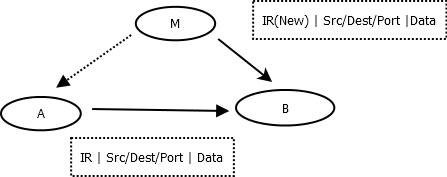
\includegraphics[scale=0.5]{falseir.png}
\caption{Demonstration of False IR attack}
\label{fig:falseir}
\end{figure}
\\
Above figure  illustrates this situation. Node A sends an IR intended for node B. Because of the broadcast medium, node M will spoof the IR and can send a changed to B as a result B will be unable to decompress compressed headers from A. But the malicious node M can still receive and decompress packets received from A  because it knows the context.\\
If the decompressor does sends feedback then it will send a NACK for the unsuccessful compressed packets. The compressor will then send a new IR header to repair the context.The malicious node will once again change the context hence the cycle will  repeat.\\
Under the False IR Attack, if the decompressor is not configured to send feedback, then this state will last for infinite time.
\subsection{False ACK attack}
Under this attack, after changing the context with a fake IR header, the malicious node sends a fake ACK to the compressor. Assuming the decompressor is configured to send feedback, it will send a NACK to this same compressed packet. As a result, the compressor will end up receiving both an ACK and a NACK for the same packet, in some order. The ROHC specification is not clear on the behavior of the compressor in this situation because this situation is never expected to happen.In that case the last feedback received will effectively overwrite the earlier feedback.\\
In the worst case, all packets unable to be decompressed by the decompressor, while the malicious
node can decompress them all. 
\subsection{False NACK attack}
alse NACK Attack (FNA) is  built-in mechanisms to re-transmit IR headers
when it receives a static negative acknowledgement (Static-NACK), indicating that the decompressor believes there is
damage to the static portion of the context. As shown in Figure\\
In this attack, the malicious node (M) simply sends false Static-NACKs to all ROHC packets received on the broadcast channel. The compressor (A) will then continue to send IR headers with each packet. As a result though the decompression occurs for one packet but compressor goes on sending the same packet.
\pagebreak



\section{Securing the library: Testing the insecurity}
This part will deal with all the setup of testing the security problems, and proving their consequences.
\subsection{Setting up the environment}
There are three nodes in the environment. A sender, a reciever and an intercepter. We use a local machines and deploy two virtual machines
to simulate the three nodes
\begin{itemize}
	\item Local Machine: The sender/broadcaster of compressed packets. Hence the compressor runs in this node.
	\item Virtual Machine A: The intended reciever of the compressed packets. Hence the decompressor runs in this node.
	\item Virtual Machine B: The interceptor. It runs its own decompressor, and captures packets and decompresses them. It might also send
	invalid feedbacks, to hamper the network or the compressor running in the local machines.
\end{itemize}

\paragraph{A note on interception} 
Virtual machines should be run in bridged mode, as opposed to NAT mode. In NAT mode, their is a virtual router that creates
its own subnet under which the virtual networks lie. This doesnot simulate a network where all the nodes
are in the same network. Hence we use bridged mode, where the virtual m/cs lie in the same network as the host. \\
Also virtual machines' promisous mode, which by default is disabled should be enabled to "Allow all".

\paragraph{A note on the compressor and decompressor mode}
The compressor-decompressor is setup to be working in O-mode (Optimistic mode). The reasoning behind this has been explained later.
Also the feedback channel has been made one way, i.e from decompressor to compressor.

\paragraph{Setting up the local machine aka the compressor}
The local machine, compresses a packet and either broadcasts it or sends it to a particular node (the virtual machine:A in this case).
The program CompressorSend which continously sends packets (or some fixed number) is structured in the following way:
\begin{itemize}
	\item Creates a compressor with a small CID (which is sufficient for testing). (Only one global compressor is needed).
	\item Sends a packet, involoving the following steps:
	\begin{enumerate}
		\item Stuffs an IP header and appends a constant payload to it.
		\item Compresses using the IP profile using the compressor created before.
		\item Sends the compressed packet over a UDP datagram.
	\end{enumerate}
	\item Listens for feedback in another channel(?) and passes the recieved feedback to the compressor
\end{itemize}

\paragraph{Setting up virtual machine:A aka the intended reciever}
The virtual machine:A is setup with a decompressor which recieves compressed packets addressed to it.
The program DecompressorRecieve which continuosly listens for a packet and decompresses it and sends feedback is structured as follows:
\begin{itemize}
	\item Creates a decompressor. (only one global decompressor)
	\item Listens for a packet
	\item For every packet recieved, extract the payload and decompress it
	\item Sends feedback to another channel(?).
\end{itemize}

\paragraph{Setting up virtual machine:B aka the interceptor}
The virtual machine:B is foremostly setup with a sniffer program which sniffs packets.
It can operate differently based on the type of attack it does. The structure of the program is thus singular, but it can be run 
in different modes(TODO):
\begin{itemize}
	\item A sniffer, that uses the pcap library to sniff packets 
	\item A feedback sender, that can send true feedback or can flood the sender with modified feedback as an attack
\end{itemize}


\subsection{



\pagebreak
\section{Securing the library: Solution}
In the following subsections, three methods in increasing level of protection against these three (False IR,False ACK,False NACK) kind of attacks are listed.
\subsection{ROHC CRC Encryption}
Most ROHC packet formats contain a cyclical redundancy check (CRC) used to detect a loss of synchronization between the compressor and decompressor. Figure  illustrates an ROHC IR header and feedback (ACK/NACK) header block with an 8-bit CRC. To produce an encrypted CRC, the compressor would first create an encrypted version of the full uncompressed header by applying some form of symmetric key encryption. The encrypted uncompressed header is then fed into the normal CRC algorithm to produce an encrypted CRC.This encrypted CRC is then used in place of a normal CRC in the compressed header.\\
The decompressor will reconstruct the original header from the compressed header, as normal. When verifying the CRC,
it will perform the additional step of applying the symmetric key to the uncompressed header before calculating the CRC.
A malicious node that does not know the key will not be able to accurately generate a CRC for a fake packet.
\subsection{IPSec encryption after compression}
The last method to protect ROHC is to utilize IPSec  to tunnel all ROHC traffic across two security associations. Using ROHC over IPsec (ROHCoIPsec), the transport layer headers (e.g., UDP, TCP,etc.) and inner IP header packets at the ingress of the IPsec tunnel are compressed and sent over the IPsec tunnel to be decompressed on the other end. Tunnel mode IPsec treats the compressed ROHC header and data as new data, and adds an ESP header and IP header to the packet, incurring an extra 28 (IPv4) to 48 (IPv6) bytes. Hence the advantage of using ROHC for compression is unachieved in this case.
\subsection{ROHC Extension for Encrypted Authentication Field}
Another option is to extend ROHC for an encrypted authentication
field. This option would add a 32 bit sequence number to protect against replay attacks, and some length of Integrity Check Value (ICV), which would be an encrypted field generated by applying a hash function to the rest of ROHC header,then encrypting the hash value using a block cipher. The size of this field can be adjusted. To enhance compression gains, the authentication fields should be included only in headers capable of changing the context state. These include Initialization and Refresh, Context Repair, and Feedback, but not normal compressed ROHC headers.


\pagebreak
\section{Securing the library: Diving in}
This part will deal with implementing the crc encryption workaround.
\end{document}

